%--------------------------------------------------------------------------------------------------%
%	The MIT License (MIT)
%
%	Copyright (c) 2015 Jan Küster
%
%	Permission is hereby granted, free of charge, to any person obtaining a copy
%	of this software and associated documentation files (the "Software"), to deal
%	in the Software without restriction, including without limitation the rights
%	to use, copy, modify, merge, publish, distribute, sublicense, and/or sell
%	copies of the Software, and to permit persons to whom the Software is
%	furnished to do so, subject to the following conditions:
%
%	THE SOFTWARE IS PROVIDED "AS IS", WITHOUT WARRANTY OF ANY KIND, EXPRESS OR
%	IMPLIED, INCLUDING BUT NOT LIMITED TO THE WARRANTIES OF MERCHANTABILITY,
%	FITNESS FOR A PARTICULAR PURPOSE AND NONINFRINGEMENT. IN NO EVENT SHALL THE
%	AUTHORS OR COPYRIGHT HOLDERS BE LIABLE FOR ANY CLAIM, DAMAGES OR OTHER
%	LIABILITY, WHETHER IN AN ACTION OF CONTRACT, TORT OR OTHERWISE, ARISING FROM,
%	OUT OF OR IN CONNECTION WITH THE SOFTWARE OR THE USE OR OTHER DEALINGS IN
%	THE SOFTWARE.
%
%
%--------------------------------------------------------------------------------------------------%


%============================================================================
%
%	DOCUMENT DEFINITION
%
%============================================================================

% Use article class to fully customize the page (do not use use a CV template)
\documentclass[10pt,x11names]{article}

\usepackage[utf8]{inputenc}
\usepackage{microtype} % improves justification

\usepackage{xifthen}  % provides \isempty test

%----------------------------------------------------------------------------------------
%	FONT
%----------------------------------------------------------------------------------------

% some tex-live fonts - choose your own

%\usepackage[defaultsans]{droidsans}
%\usepackage[default]{comfortaa}
%\usepackage{cmbright}
%\usepackage[default]{raleway}
%\usepackage{fetamont}
\usepackage[default]{gillius}
%\usepackage[light,math]{iwona}
%\usepackage[thin]{roboto}

% set font default
\renewcommand*\familydefault{\sfdefault}

\usepackage{moresize}     % more font size definitions
\usepackage{fontawesome5}%\faStyle{regular} % [solid (default), regular]
\usepackage{emoji}
\usepackage{tabularx}
\usepackage[normalem]{ulem} % [normalem] prevents the package from changing the default behavior of `\emph` to underline.

%----------------------------------------------------------------------------------------
%	PAGE LAYOUT  DEFINITIONS
%----------------------------------------------------------------------------------------

%debug page outer frames
%\usepackage{showframe}

% ADJUST PAGESIZE
% define page size and styles using geometry
\usepackage[paperheight=442.5mm, paperwidth=230mm]{geometry} % [a4paper] [heightrounded]???

% for example, change the margins to 2 inches all round
\geometry{top=0.8cm, bottom=-.6cm, left=0.4cm, right=1cm}

% less space between header and content
\setlength{\headheight}{-5pt}

%indentation is zero
\setlength{\parindent}{0mm}

%----------------------------------------------------------------------------------------
%	TABLE /ARRAY DEFINITIONS
%----------------------------------------------------------------------------------------

% Layouting tables
\usepackage{multicol}
\usepackage{multirow}

% Extended aligning of tabular cells
\usepackage{array}

\newcolumntype{x}[1]{%
>{\raggedleft\hspace{0pt}}p{#1}}%

%----------------------------------------------------------------------------------------
%	GRAPHICS DEFINITIONS
%----------------------------------------------------------------------------------------

\usepackage{graphicx}

% For floating figures
\usepackage{wrapfig}
\usepackage{float}
%\floatstyle{boxed}
%\restylefloat{figure}

% For drawing graphics
\usepackage{tikz}
\usetikzlibrary{shapes, backgrounds, mindmap, trees, positioning, shadings}

% Bubble diagrams
\usepackage{smartdiagram}
\smartdiagramset{
    bubble center node font = \footnotesize,
    bubble node font = \footnotesize,
    % specifies the minimum size of the bubble center node
    bubble center node size = 0.5cm,
    %  specifies the minimum size of the bubbles
    bubble node size = 0.9cm,
    % specifies which is the distance among the bubble center node and the other bubbles
    distance center/other bubbles = 0.5cm,
%     % sets the distance from the text to the border of the bubble center node
%     distance text center bubble = 0.5cm,
%     % set center bubble color
%     bubble center node color = pastelblue,
%     % define the list of colors usable in the diagram
%     set color list = {lightgray, materialcyan, orange, green, materialorange, materialteal, materialamber, materialindigo, materialgreen, materiallime},
%     % sets the opacity at which the bubbles are shown
%     bubble fill opacity = 0.6,
%     % sets the opacity at which the bubble text is shown
%     bubble text opacity = 1,
}

%----------------------------------------------------------------------------------------
%	Color DEFINITIONS
%----------------------------------------------------------------------------------------

\usepackage{transparent}
\usepackage{xcolor}

% Accent color
\definecolor{complcol}{RGB}{250,150,10}

% Light background
\definecolor{softcol}{RGB}{225,225,225}

% Custom colors
\definecolor{pastelblue}{HTML}{0395DE}
\definecolor{customblue1}{HTML}{428bca}

\definecolor{scala2blue}{HTML}{e45c77}
\definecolor{scala3rose}{HTML}{5cc6e4}
% From the \lambda Haskell logo (L to R): 453a62 5e5086 8f4e8b <- purples,  3f3f3f <- gray
\definecolor{haskell1}{HTML}{453a62}
\definecolor{haskell2}{HTML}{5e5086}
\definecolor{haskell3}{HTML}{8f4e8b}
\definecolor{haskell4}{HTML}{3f3f3f}

\definecolor{haskellweb1}{HTML}{3d1f54}
\definecolor{haskell2custom1}{HTML}{5a4b82}
\definecolor{haskell2custom2}{HTML}{5b4796}

% --vvv-- Color schemes --vvv--

% Bright brown/blue
% \colorlet{bgcol}{Sienna3}
% \colorlet{sectcol}{DodgerBlue1}
% \colorlet{sidecolor}{DodgerBlue3}
% \colorlet{introcolor}{bgcol}

% Pale gray/blue
% \colorlet{bgcol}{Ivory4}
% \colorlet{sectcol}{customblue1}
% \colorlet{sidecolor}{sectcol}
% \colorlet{introcolor}{bgcol}

% Scala2/3 schema (like)
% \colorlet{bgcol}{scala3rose}
% \colorlet{sectcol}{scala2blue}
% \colorlet{sidecolor}{scala2blue}
% \colorlet{introcolor}{bgcol}

% Haskell schema
\colorlet{bgcol}{haskellweb1}
\colorlet{sectcol}{haskell2custom1}
\colorlet{sidecolor}{haskell4}
\colorlet{introcolor}{haskell3}

% Package for links, must be the last package used
\usepackage[
  colorlinks = true,
%   linkcolor = blue,
%   urlcolor = blue,
%   citecolor = blue,
%   anchorcolor = blue,
]{hyperref}

%============================================================================%
%
%
%	DEFINITIONS
%
%
%============================================================================%

% Returns minipage width minus two times \fboxsep
% to keep padding included in width calculations
\newcommand{\mpwidth}{\linewidth-\fboxsep-\fboxsep}

%----------------------------------------------------------------------------------------
% 	ARROW GRAPHICS in Tikz
%----------------------------------------------------------------------------------------

% a six pointed arrow poiting to the left
\newcommand{\tzlarrow}{(0,0) -- (0.2,0) -- (0.3,0.2) -- (0.2,0.4) -- (0,0.4) -- (0.1,0.2) -- cycle;}

% include the left arrow into a tikz picture
% param1: fill color
%
\newcommand{\larrow}[1]
{\begin{tikzpicture}[scale=0.58, every path/.style={rounded corners=0pt}] % reset style to avoid inherited rounded from outer tikzpicture
	\filldraw[fill=#1!100,draw=#1!100!black]  \tzlarrow
 \end{tikzpicture}
}

% a six pointed arrow pointing to the right
\newcommand{\tzrarrow}{ (0,0.2) -- (0.1,0) -- (0.3,0) -- (0.2,0.2) -- (0.3,0.4) -- (0.1,0.4) -- cycle;}

% include the right arrow into a tikz picture
% param1: fill color
%
\newcommand{\rarrow}
{\begin{tikzpicture}[scale=0.7]
	\filldraw[fill=sectcol!100,draw=sectcol!100!black] \tzrarrow
 \end{tikzpicture}
}

% =====================
% === Customization ===
% =====================

% Custom command to specify the color in links
\newcommand*{\hrefcol}[3][magenta]{\href{#2}{\textcolor{#1}{#3}}}

%----------------------------------------------------------------------------------------
%	custom sections
%----------------------------------------------------------------------------------------

% create a coloured box with arrow and title as cv section headline
% param 1: section title
%
\newcommand{\cvsection}[1]{
  \colorbox{sectcol}{\mystrut \makebox[1\mpwidth][l]{
  \larrow{introcolor!70!white} \hspace{-8pt} \larrow{introcolor!40!white} \hspace{-8pt} \larrow{introcolor!10!white} \textbf{\textcolor{white}{\uppercase{#1}}}\hspace{4pt}
  }}\\
}

% create a coloured arrow with title as cv meta section section
% param 1: meta section title
%
\newenvironment{metasection}[1] {
	\vspace{6pt}
	\begin{center}
		\textcolor{white}{\large{\uppercase{#1}}}\\
	\normalsize
	\parbox{0.7\mpwidth}{\textcolor{white}	\hrule}
}{\end{center}}

%----------------------------------------------------------------------------------------
%	 CV ENTRIES: cvposition, cventry, cvevent (the original one)
%----------------------------------------------------------------------------------------

% Company/position heading command
% arg1: dates
% arg2: position
% arg3: company
\newcommand{\cvposition}[3]{
  \begin{tabular*}{1\mpwidth}{@{\hskip 1pt} p{0.575\mpwidth}  x{0.41\mpwidth}}
    \textcolor{black}{\textbf{#2}} & \textcolor{complcol}{#3}, \textcolor{gray}{#1}
  \end{tabular*}
  \textcolor{softcol}{\hrule}
  \vspace{6pt}
}

\newcommand{\cventry}[1]{
  \begin{minipage}[t]{0.04\mpwidth}
    \hspace{3pt}\larrow{softcol}
  \end{minipage}
  \begin{minipage}[t]{0.97\mpwidth}
    #1\\[-5pt]
  \end{minipage}
  %\par
  %\vspace{5pt}
}

% creates a stretched box as cv entry headline followed by two paragraphs about
% the work you did
% param 1:	event time i.e. 2014 or 2011-2014 etc.
% param 2:	event name (what did you do?)
% param 3:	institution (where did you work / study)
% param 4:	what was your position
% param 5:	some words about your contributions
%
\newcommand{\cvevent}[5]
{
\vspace{8pt}
	\begin{tabular*}{1\mpwidth}{p{0.55\mpwidth}  x{0.42\mpwidth}}
 	\textcolor{black}{\textbf{#2}} & \textcolor{complcol}{#3}, \textcolor{bgcol}{#1}

	\end{tabular*}
\vspace{-12pt}
\textcolor{softcol}{\hrule}
\vspace{6pt}
	\begin{tabular*}{0.5\mpwidth}{p{\mpwidth}}
\larrow{softcol}  #4\\[3pt]
\larrow{softcol}  #5\\[6pt]
	\end{tabular*}
}

% creates a stretched box as
\newcommand{\cveventmeta}[2]
{
	\mbox{\mystrut \hspace{87pt}\textit{#1}}\\
	#2
}

% Macro for impact generated 🎯
\newcommand{\cvimpact}[1]{
  \parbox{\mpwidth}{
    \emoji{bullseye} \emph{#1}
  }
  \vspace{5pt}
}

%----------------------------------------------------------------------------------------
% CUSTOM STRUT FOR EMPTY BOXES
%----------------------------------------- -----------------------------------------------
\newcommand{\mystrut}{\rule[-.3\baselineskip]{0pt}{\baselineskip}}

%----------------------------------------------------------------------------------------
% CUSTOM LOREM IPSUM
%----------------------------------------------------------------------------------------
\newcommand{\lorem}{Lorem ipsum dolor sit amet, consectetur adipiscing elit. Donec a diam lectus.}

% use to vertically center content
% credits to: http://tex.stackexchange.com/questions/7219/how-to-vertically-center-two-images-next-to-each-other
\newcommand{\vcenteredinclude}[1]{\begingroup
\setbox0=\hbox{\includegraphics{#1}}%
\parbox{\wd0}{\box0}\endgroup}

% use to vertically center content
% credits to: http://tex.stackexchange.com/questions/7219/how-to-vertically-center-two-images-next-to-each-other
\newcommand*{\vcenteredhbox}[1]{\begingroup
\setbox0=\hbox{#1}\parbox{\wd0}{\box0}\endgroup}

%----------------------------------------------------------------------------------------
%	ICON MACROS
%----------------------------------------------------------------------------------------

% args: (iconName, boxSize, color)
\newcommand{\icon}[3]{%                 %icon shortcut
    \vcenteredhbox{\makebox(#2, #2){\textcolor{#3}{\faIcon{#1}}}}%
}

% args: (iconName, boxSize, text, color)
\newcommand{\icontext}[4]{% 						%icon with text shortcut
    \vcenteredhbox{\icon{#1}{#2}{#4}} \vcenteredhbox{\textcolor{#4}{#3}}%
}

% args: (iconName, boxSize, text, url, textColor)
\newcommand{\iconhref}[5]{% 					  %icon with website url
    \vcenteredhbox{\icon{#1}{#2}{#5}} \href{#4}{\textcolor{#5}{#3}}%
}

% args: (iconName, boxSize, text, mailto, color)
\newcommand{\iconemail}[5]{% 					  %icon with email link
    \vcenteredhbox{\icon{#1}{#2}{#5}} \href{mailto:#4}{\textcolor{#5}{#3}}%
}

%----------------------------------------------------------------------------------
%  Fork me on GitHub
%----------------------------------------------------------------------------------

%\usepackage{tikz} % already included
\usepackage{ifthen}
%\usepackage{xcolor} % already included
\usetikzlibrary{shadows.blur}

\definecolor{forkmebg}{HTML}{3873b3}
\definecolor{forkmefg}{HTML}{eeeeee}

% rotate and shift are hardcoded here because of the href workaround, see also https://gist.github.com/dokenzy/fe8967c8a5921191a261
\newcommand{\forkme}{
  \begin{tikzpicture}[remember picture, overlay]
    \node[rotate=-50, shift={(-1.7cm, -1.7cm)}] at (current page.north east) {
      \begin{tikzpicture}[remember picture, overlay]
        \node[fill=forkmebg, text centered, minimum width=50em, minimum height=2.3em, blur shadow, shadow yshift=0pt, shadow xshift=0pt, shadow blur radius=.4em, shadow opacity=50](fmogh) at (0pt, 0pt) {}; % workaround: text/link see below
        \draw[forkmefg!60, dashed, line width=.08em, dash pattern=on .5em off 1.5\pgflinewidth] (-25em,0.9em) rectangle (25em,-0.9em);
      \end{tikzpicture}
    };
    % workaround: the link needs to be defined using a \rotatebox{deg} because \node[rotate=deg]{\href} isn't rendered correctly
    \node[shift={(-1.10cm, -1.35cm)}, text centered, minimum width=50em, minimum height=3.0em, text=forkmefg](fmogh) at (current page.north east) {\fontfamily{phv}\selectfont\bfseries \href{https://github.com/gerardbosch/resume}{\rotatebox{-50}{\color{white}{\small Fork me on GitHub}}} };
  \end{tikzpicture}
}

%============================================================================
%
%	DOCUMENT CONTENT
%
%============================================================================

\begin{document}
\fcolorbox{white}{white}{\begin{minipage}[b][0.974\textheight][t]{0.71\linewidth}


%---------------------------------------------------------------------------------------
%	TITLE HEADLINE
%----------------------------------------------------------------------------------------

\vspace{-3pt}
\colorbox{bgcol}{\color{white}\makebox[\mpwidth][c]{
  \hspace{46pt}\HUGE{\uppercase{Gerard Bosch} }
  \textcolor{introcolor}{\rule[-1mm]{1mm}{0.9cm}}
  \parbox[b]{5cm}{
    \large{{Software Engineer}} \\
    {{Freelancer/Contractor}}
  }
}}

%----------------------------------------------------------------------------------------
%	HEADER IMAGE / BANNER
%----------------------------------------------------------------------------------------

\begin{minipage}[b][45.1mm][t]{\linewidth} % Fixed-size container
  \begin{tikzpicture}[remember picture, overlay]

    % introcard style def
    \tikzstyle{introcard}=
        [ anchor=north west, inner sep=4pt
        , text width=79mm, align=center
        , rounded corners=5pt
        , opacity=0.82, text opacity=1
        , left color=introcolor, right color=introcolor!62!white, text=white
        % , right color=introcolor, left color=introcolor!58!white, text=white
        % , fill=white, text=black
        ]

    % Background image
    \node[anchor=north west, inner sep=0] at (0,0) {
      % 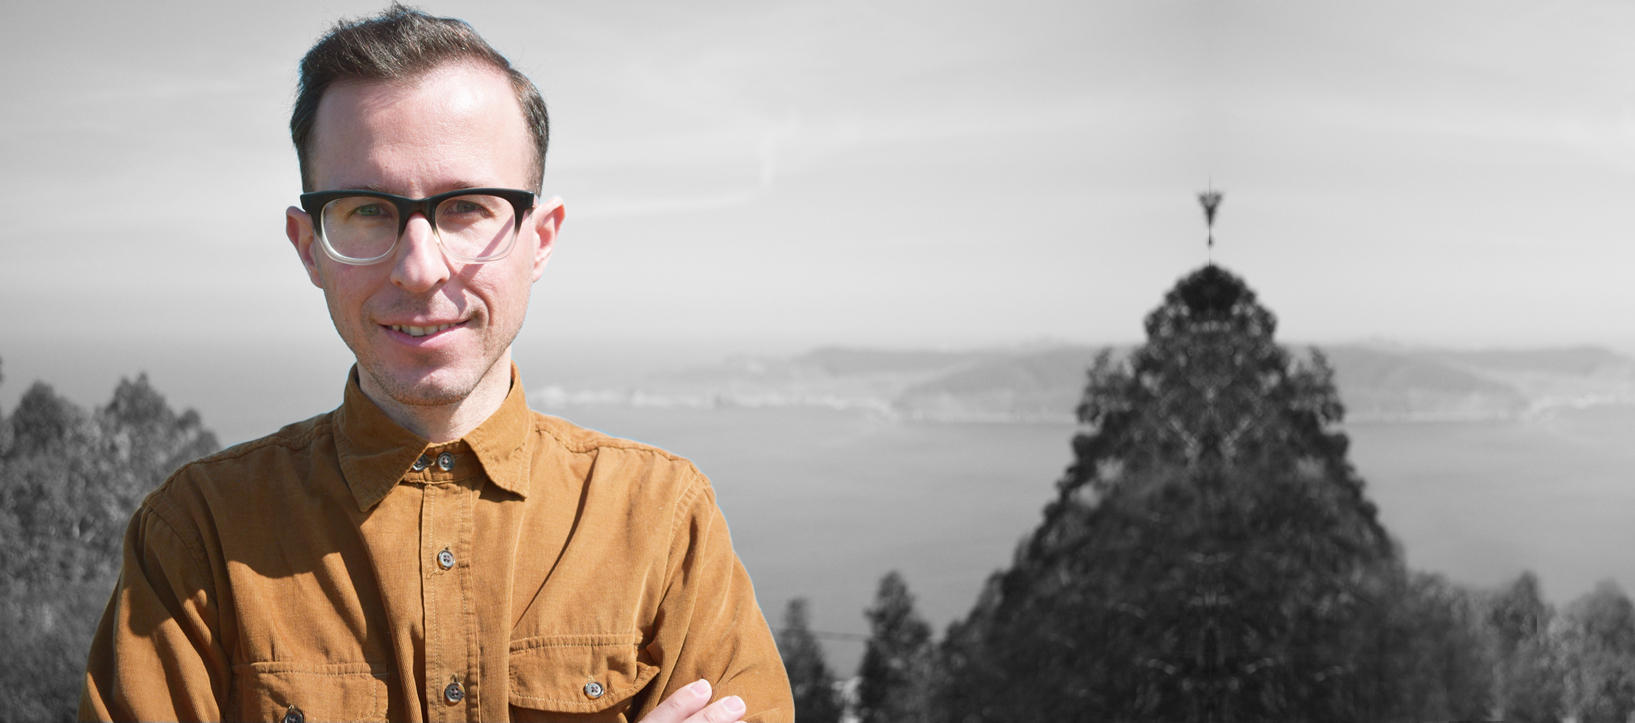
\includegraphics[trim=0 30 0 10, clip, width=\linewidth]{header-mountain_75.jpg} % Galicia
      
\includegraphics[trim=28 25 0 98, clip, width=173mm]{header-flatiron_75.jpg} % Flatiron NY
    };

    % Color box node relative to the minipage top left
    \node[introcard] at (68mm, -6mm) {
      \setlength{\spaceskip}{2pt} % compact text a little

      \larrow{sectcol}
      Enthusiast about Functional Programming, software engineering/craftsmanship, clean code, architectural/ design patterns and programming languages theory.\vspace{1pt}
    };

    % Color box node relative to the minipage top left
    \node[introcard] at (68mm, -25mm) {
      \setlength{\spaceskip}{2pt} % compact text a little

      \larrow{sectcol}{% keep block here `{` and end vspace => better text arrangement
        Good at identifying inefficiencies, \textcolor{Gold1}{finding solutions} and \textcolor{Gold1}{improving processes}. I enjoy collaborating with diverse teams to solve challenging problems.
      }
      \vspace{1pt}
    };
  \end{tikzpicture}
\end{minipage}


%---------------------------------------------------------------------------------------
%	INTRODUCTION
%----------------------------------------------------------------------------------------

\transparent{0.85} % this transparency makes everything more lightweight and kind, specially big paragraphs :)

%============================================================================%
%
%	CV SECTIONS AND EVENTS (MAIN CONTENT)
%
%============================================================================%

%---------------------------------------------------------------------------------------
%	SUMMARY
%----------------------------------------------------------------------------------------
\cvsection{Summary}

[ \emoji{ledger}\emoji{eyes} \textcolor{gray}{\emph{Read more about \href{https://mnf.red/gerardbosch}{my best practices} and skills}} | \emoji{scroll} \textcolor{gray}{\emph{Read the \href{https://cv.gerardbosch.xyz}{extended CV} version}} ]

\vspace{12pt}
\parbox{\mpwidth}{{\small
  With a keen interest in Scala and other modern functional languages, my background is mostly about designing/implementing backend systems and APIs. Skilled in analyzing requirements and translating them into code. Focused on code readability, expressiveness, precision, conciseness, and correctness. Committed to continuous improvement \& continuous refactor and code reuse as a mantra. Accidental-complexity fighter. Curious by nature, proactive and self-taught. I enjoy contributing to developer experience and building products. Like learning~\emoji{smiley}, love crafting \emoji{heart}.
}}

\vspace{12pt}

%---------------------------------------------------------------------------------------
%	EXPERIENCE
%----------------------------------------------------------------------------------------
\cvsection{Experience}

% Original cvevent example
%\cvevent{2020 - now}{}{}{}{}
%\textcolor{softcol}{\hrule}

% New custom commands below :)

\cvposition{2024--2025}{Backend Software Engineer | Quarkus, Reactive}{Tymit}

\cvimpact{
  Authored an RFC with actionable proposals to align the current architecture with Clean Architecture™ \& SOLID principles, with a special focus on the Interface Segregation (ISP) and Single Responsibility Principle (SRP), plus other enhancements.
}

\cventry{
  Engaged with the integrations team to support the migration of hundreds of thousands of customers into our system, while also developing new public-facing APIs to enable a new business model requiring first-party and third-party B2B backend integrations.
}
\null
\cventry{
  Improved testing reliability by introducing Property-Based Testing and showcasing its principles to the backend team, ensuring more robust testing including edge-cases, generating thousands of test values.
}
\null
\cventry{
  Spearheaded API contract segregation into dedicated modules, enabling the publication of versioned API artifacts for seamless and efficient cross-service integration using Gradle, contributing to DX.
}
\null
\cventry{
  Shared coding best practices and actively contributed to code reviews and BE discussions.
}
\null

% \vspace*{3pt}
~\textbf{Stack}: \textit{Quarkus, Microservices, Reactive Programming, AWS (ECS, DynamoDB, SQS, SNS, RDS), Liquibase,\ldots}

\vspace{1em}
\cvposition{2022--2023}{Software Engineer | C++, MQL}{Self employed}

\cvimpact{
  Established my own company to provide software engineering services as a contractor.
}

\cventry{
  Algorithmic trading, research, design \& implementation of a risk management system for loss control, as well as key metrics collection/reporting using DDD \& Hexagonal arch.
}
\null
\cventry{
  High level design of a multi-level affiliation system with referral fee distribution.
}
\null
\cventry{
  Took a break to learn about finances, markets, investments and expand Fintech expertise.
}
\null

\vspace{1em}
\cvposition{2021--2022}{Software Engineer | Spring Boot, Kotlin}{N26 Bank}

\cvimpact{
  Collaborated to streamlining the processing of banking fees with the goal of having a more centralized and clear domain boundaries for charging fees.
}

\cventry{
  Joined the Memberships team, which was in charge of designing and operating a new fee platform intended to be the new-standardized way of charging company-wide banking fees.
}\null
\cventry{
  This involved creating a dedicated microservice, repurposing and refactoring of existent ones (by DDD/CleanArch), along with APIs, as well as DB migrations.
}\null
\cventry{
  Being a bank, testing and security were some of the most important and cared matters (pyramid testing, contract testing, regression, TDD,\ldots).
}\null

\vspace*{3pt}~\textbf{Stack}: \textit{Kotlin, Spring Boot, Microservices, EDA, Kafka, REST, Postgres, Datadog, ELK, AWS,\ldots}

\vspace{1em}
\cvposition{2016--2021}{Senior Software Engineer | Spring Boot, Java}{GFT IT Consulting}

% ~~PROJECT HIGHLIGHTS (most relevant ones):

\cvimpact{
  Successfully delivered a large and complex regulatory banking project to provide external, permission-based access to banking APIs, ensuring on-time completion. Then, was called to contribute to building a new bank architecture for high-concurrency from the acquired know-how.
}

\cventry{
  \textit{Banc Sabadell}: \textbf{Middleware Architecture} (2020--2021) --
  Redefine from scratch a whole new framework and development environment based on MsA, Spring Boot, API-First, Event Driven, DDD, Hexagonal, and using OKR project framework
  -- \textbf{Role}: Software Engineer.
}
\null
\cventry{
  \textit{Banc Sabadell}: \textbf{PSD2 \& APIfication} (2018--2020) --
  Design \& implement the APIs and requirements for the European \href{https://en.wikipedia.org/wiki/Payment_Services_Directive}{PSD2 regulation}; pioneering the API exposition for the Bank.
  Define and implement architectural components for the MsA.
  Mentoring and onboarding new members. Got established as the technical lead for the dev team
  -- \textbf{Role}: Tech Lead.
}
\null
\cventry{
  \textit{Bankinter}: \textbf{Microservice Architecture} (2017) --
  Development of an architecture based on MsA and Spring, providing the pre-configured components: from security, tracing, audit, error handling to cryptography; enabling developers to easily get started.
}


\vspace{1em}
\cvposition{2015--2016}{Software Engineer | Mobile development}{ICG Software}

\cventry{
  Developed a new Android-native warehouse management app, featuring barcode scanning, offline operation, an object database with Realm, and integration with the in-house developed ERP.
}
\null
\cventry{
  Successfully migrated a whole app for a franchise clothing store to native Windows Phone. Our client needed that we developed our Android app for Windows Phone, to deploy it globally on all their stores.
}

\vspace{1ex}
\cvposition{2012--2013}{Researcher/developer | Python}{AI Research Institute IIIA-CSIC}
%~~Spanish National Research Council. Innpacto-2011 (Spanish Science and Innovation Ministry),\par\vspace{2pt}
~~\emph{NEWMATICA: Intelligent and Energy Efficient Advanced System for Vacuum Waste Collection}.\\[3pt]
\cventry{Investigated Machine Learning algorithms based on \emph{Approximate Dynamic Programming} (RL).}\\
\cventry{Co-developed a waste collecting simulator to optimize operational plans, run simulations, collect data and process results.}

\vspace{1ex}
\hspace{1pt}\textbf{Presentations} \\[-2ex] \textcolor{softcol}{\hrule}\vspace{6pt}

\begin{tabular}{cl}
    2020 & \href{https://bit.ly/fp-short-intro}{Functional Programming super-short intro} \\
    2018 & \href{https://blockchain-presentation.gerardbosch.xyz}{A technical introduction to Blockchain technology} \\
\end{tabular}\vspace{5pt}


%---------------------------------------------------------------------------------------
%	EDUCATION SECTION
%---------------------------------------------------------------------------------------
\cvsection{Education ~\lowercase{\emph{(to see more, view the \href{https://cv.gerardbosch.xyz}{\color{magenta}{CV version}})}}}

\vspace{-5pt}
\cvposition{2011}{M.Sc. Open Source Software Eng.}{University of Lleida (ES) / VIA UC (DK)}
\cventry{Master Thesis: \emph{Setting up and deployment of Sauron system for DNS system management at University of Lleida}. Mobility internship program at \emph{VIA UC}, Denmark.}

% \cvposition{2010}{Bachelor Computer Science}{University of Lleida}\vspace{-2pt}
% \cventry{Bachelor Thesis: \emph{Implementation of Golay codes in Sage Math.}}


%---------------------------------------------------------------------------------------
%	LIVE RESUME NOTE
%---------------------------------------------------------------------------------------
% \vfill\vspace{3pt}
% \centerline{
%   \href{https://resume.gerardbosch.xyz}{\emoji{person-gesturing-ok} \textcolor{black}{This \emph{résumé} is \textcolor{magenta}{live!} Click here to ensure you access the most \textbf{up-to-date} version \emoji{person-gesturing-ok}}}
% }

\end{minipage}}%
\fcolorbox{white}{sidecolor}{\begin{minipage}[b][0.974\textheight][t]{0.31\linewidth}


%----------------------------------------------------------------------------------------
%	SIDE BAR
%----------------------------------------------------------------------------------------

\begin{metasection}{Contact}

	\icontext{globe-americas}{12}{US/EU Worldwide remote}{white}\\[5pt]
	%\icontext{MobilePhone}{12}{}{white}\\[5pt]
	\iconemail{envelope}{12}{gerard.bosch@gmail.com}{gerard.bosch@gmail.com}{white} \\[5pt]
	\iconhref{linkedin}{12}{linkedin.com/in/gerard-bosch}{https://www.linkedin.com/in/gerard-bosch}{white} \\[5pt]
	%\iconhref{MousePointer}{12}{Webpage}{Webpage}{white} \\[5pt]
	\iconhref{github-alt}{12}{github.com/gerardbosch}{https://github.com/gerardbosch}{white} \\[5pt]
	%\iconhref{StackOverflow}{12}{stackoverflow.com/users/6108874/gerard-bosch}{https://stackoverflow.com/users/6108874/gerard-bosch}{white} \\[5pt]
	%\iconhref{Twitter}{12}{@user}{https://twitter.com/user}{white} \\[5pt]
  \iconhref{laptop}{12}{gerardbosch.xyz}{https://gerardbosch.xyz}{white} \\[5pt]
\end{metasection}

\vspace{-0.3cm}
\begin{metasection}{Programming Lang}\color{white}
\vspace{5pt}
\begin{tabular}{rl}

Scala 3 &
\icon{star}{12}{complcol}\icon{star}{12}{complcol}\icon{star}{12}{complcol}\icon{star}{12}{white}\icon{star}{12}{white} \\[2pt]

Kotlin &
\icon{star}{12}{complcol}\icon{star}{12}{complcol}\icon{star}{12}{complcol}\icon{star}{12}{complcol}\icon{star}{12}{white} \\[2pt]

Java 23 &
\icon{star}{12}{complcol}\icon{star}{12}{complcol}\icon{star}{12}{complcol}\icon{star}{12}{complcol}\icon{star}{12}{complcol} \\[2pt]

Haskell &
\icon{star}{12}{complcol}\icon{star}{12}{complcol}\icon{star}{12}{white}\icon{star}{12}{white}\icon{star}{12}{white} \\[2pt]

Bash &
\icon{star}{12}{complcol}\icon{star}{12}{complcol}\icon{star}{12}{complcol}\icon{star}{12}{complcol}\icon{star}{12}{white} \\[2pt]

Python &
\icon{star}{12}{complcol}\icon{star}{12}{complcol}\icon{star}{12}{complcol}\icon{star}{12}{white}\icon{star}{12}{white} \\[2pt]

Perl &
\icon{star}{12}{complcol}\icon{star}{12}{white}\icon{star}{12}{white}\icon{star}{12}{white}\icon{star}{12}{white}

\end{tabular}
\end{metasection}


\vspace{-0.3cm}
\begin{metasection}{Technologies}

% \color{white}{\faDatabase~SQL} % alternative way, produces better vertical alignment than the custom \icontext
\icontext{code}{12}{Spring Boot}{white}~
\icontext{code}{12}{Vavr}{white}~
\icontext{key}{12}{oAuth/JWT}{white} \\[5pt]

\icontext{cloud}{12}{Cloud-Native / AWS}{white}~
\icontext{docker}{12}{Docker}{white} \\[5pt]

\icontext{database}{12}{SQL}{white}~
\icontext{puzzle-piece}{12}{API First \& OpenAPI}{white} \\[5pt]

\icontext{cubes}{12}{OpenShift}{white}~
\icontext{cloudflare}{12}{Cloudflare}{white} \\[5pt]

\icontext{cube}{12}{Devcontainers}{white}~
\icontext{cube}{12}{Testcontainers}{white} \\[5pt]


\icontext{gavel}{12}{Maven/Gradle/sbt}{white}~
\icontext{life-ring}{12}{JGitVer}{white}% \\[5pt]

\end{metasection}


\vspace{-0.3cm}
\begin{metasection}{Tools}

\icontext{code}{12}{IntelliJ / VSCode / vim :)}{white} \\[5pt]
\icontext{github}{12}{GitHub Actions}{white} \icontext{gitlab}{12}{GitLab CI}{white} \icontext{jenkins}{12}{Jenkins}{white} \\[5pt]
\icontext{code-branch}{12}{Git}{white}~ \icontext{terminal}{12}{ZSH}{white}~ \icontext{comment}{12}{Codestream}{white} \\[5pt]
\icontext{rocket}{12}{CI/CD}{white}~ \icontext{linux}{12}{Linux}{white}~ \icontext{dropbox}{12}{Nix}{white}

\end{metasection}


\vspace{-0.3cm}
\begin{metasection}{Methodologies}

\begingroup\color{white}
\begin{itemize}
  \item Agile, OKR, SCRUM, Kanban
  \item TDD, Property-Based Testing, Mutation Testing
  \item Domain Driven Design, Hexagonal, Clean Architecture
  \item API-First, OpenAPI, API Management
  \item Microservices, Event-Driven Architecture
  \item SOLID, Design Patterns, Refactoring,\\ eXtreme Programming
\end{itemize}
% eXtreme Programming, Programming with types.
\endgroup
\end{metasection}

% \begin{metasection}{Activities}
%
% \textcolor{white}{\LARGE{\icon{Gamepad}{24}{white} \icon{Headphones}{24}{white}  \icon{Bicycle}{24}{white}}}
% \end{metasection}
%
% \begin{metasection}{Operating Systems}
%
% \textcolor{white}{\LARGE{\icon{Linux}{24}{white} \icon{Apple}{24}{white}  \icon{Windows}{24}{white}}}
%
% \end{metasection}

%---------------------------------------------------------------------------------------
%	Knowledge Areas
%----------------------------------------------------------------------------------------

\vspace{-0.3cm}
\begin{metasection}{In graphics...}
\begin{center}

\vspace{1ex}
\smartdiagramset{
    bubble center node font = \footnotesize,
    bubble node font = \footnotesize,
    % specifies the minimum size of the bubble center node
    bubble center node size = 0.1cm,
    %  specifies the minimum size of the bubbles
    bubble node size = 0.9cm,
    % specifies which is the distance among the bubble center node and the other bubbles
    distance center/other bubbles = 0.5cm,
    % sets the distance from the text to the border of the bubble center node
    %distance text center bubble = 0.5cm,
    % set center bubble color
    bubble center node color = pastelblue,
    % define the list of colors usable in the diagram
    %set color list = {lightgray, materialcyan, orange, green, materialorange, materialteal, materialamber, materialindigo, materialgreen, materiallime},
    % sets the opacity at which the bubbles are shown
    %bubble fill opacity = 0.6,
    % sets the opacity at which the bubble text is shown
    %bubble text opacity = 1,
}
\smartdiagram[bubble diagram]{
    Knowledge \\ Areas,
    \normalsize{\textbf{Functional}} \\ \normalsize{\textbf{Programming}},
    DevOps,
    \textbf{Distributed} \\ \textbf{Systems},
    Reactive \\ Programming,
    \normalsize{\textbf{~~Design~~}} \\ \normalsize{\textbf{patterns}},
    \normalsize{\textbf{API design}} \\ \normalsize{\textbf{\& Tooling}},
    \textbf{Architectural} \\ \textbf{patterns},
    API\\ security
}

\vspace{3ex}
\begin{tikzpicture}
  % Define styles for the nodes: planet, satellite, satchild
  \tikzstyle{planet}=[circle, fill=orange, minimum size=3.2cm, align=center]
  \tikzstyle{satellite}=[circle, draw, fill=green!40, minimum size=1.85cm, inner sep=0pt, align=center, opacity=0.7, font=\footnotesize, postaction={draw=white, line width=1.5pt, opacity=1}]
  \tikzstyle{satchild}=[circle, draw, fill=green!20, minimum size=0.7cm, inner sep=3pt, align=center, opacity=0.7, font=\footnotesize, postaction={draw=white, line width=1pt, opacity=1}]

  \node (interests) [planet] {Interest \\ Areas};

  \node (ai) [satellite, fill=yellow!30] at ($(interests)+(30:2.2cm)$) {\textbf{Artificial} \\ \textbf{Intelligence}};
  \node (blockchain) [satellite, fill=blue!30] at ($(interests)+(90:2.2cm)$) {\textbf{DLTs/} \\ \textbf{Blockchain,} \\ \textbf{Web3}};
  \node (wasm) [satellite, fill=cyan!30] at ($(interests)+(150:2.2cm)$) {\scriptsize{\textbf{WebAssembly}} \\ \textbf{(Wasm)}};
  \node (durable) [satellite, fill=Plum2!30] at ($(interests)+(210:2.2cm)$) {\hrefcol[violet]{https://www.golem.cloud/post/what-is-durable-computing}{\parbox{1.4cm}{\centering \dashuline{\bfseries Durable\\\bfseries Computing}}}};
  \node (fp) [satellite, fill=green!40] at ($(interests)+(270:2.2cm)$) {\textbf{Functional} \\ \textbf{Programming}};

  \node (unison) [satchild] at ($(fp)+(215:1.4cm)$) {\hrefcol[violet]{https://www.unison-lang.org/docs/the-big-idea/}{\dashuline{Unison}}};
  \node (effectsystems) [satchild] at ($(fp)+(270:1.4cm)$) {Effect\\ systems};
  \node (zio) [satchild] at ($(fp)+(325:1.5cm)$) {
    \hrefcol[violet]{https://zio.dev/}{\dashuline{ZIO}},\\
    \hrefcol[violet]{https://getkyo.io}{\dashuline{Kyo}},
    \hrefcol[violet]{https://ox.softwaremill.com}{\dashuline{Ox}}
  };

  \node (bigdata) [satellite, fill=gray!30] at ($(interests)+(330:2.2cm)$) {\scriptsize{\textbf{Big/Fast Data}} \\ \scriptsize{\textbf{\& Streaming,}} \\ \scriptsize{\textbf{Event-Driven}}};
\end{tikzpicture}

\end{center}
\end{metasection}


%%%%%%%%%%%%%%%%%%%%%%%%%%%%%%%%%
\end{minipage}}    % end side bar
%%%%%%%%%%%%%%%%%%%%%%%%%%%%%%%%%

% Fork me on GitHub
% \scalebox{.9}{\forkme}
\forkme

%-------------------------------------------------------------------------------------------------
%	ARTIFICIAL FOOTER (fancy footer cannot exceed linewidth)
%--------------------------------------------------------------------------------------------------

\vspace{-3pt}
\hspace{-0.25\linewidth}\colorbox{bgcol}{\makebox[1.5\linewidth][c]{
  \mystrut \small \textcolor{white}{
    \hspace{9pt}\LaTeX~source of this \textit{résumé} is available at {\normalsize\faGithub}~\href{https://github.com/gerardbosch/resume}{\color{white}{github.com/gerardbosch/resume}}~$\cdot$~Built/Delivered by GH Actions/Cloudflare~$\cdot$~Last updated: February 25, 2025
  }
}}

%============================================================================%
%
%	DOCUMENT END
%
%============================================================================%
\end{document}
